\chapter{Experiment: agent training and simulation}
Chapters 4 and 5 focus on the experimental phase of our project. This chapter details the training procedure of our SAC agent for the swing-up task and then transitions to a simulation phase to validate results for both the swing-up and stabilization tasks. We have structured this chapter into three distinct subsections: training setup, training process, and simulation results.

The first subsection describes the foundation of a reinforcement learning interaction rooted in a stable baseline3-based RL algorithm. It also touches upon a customized environment inherited from the OpenAI Gym environment. The second subsection centers on hyperparameter tuning and highlights the challenges encountered during training. The third subsection displays the results acquired from both the pendubot and acrobot setups.
\section{Training setup}
This section is about training setup and environemnt building.
\begin{figure}[htbp]
    \centering
    \includegraphics[width=0.7\linewidth]{example-image}
    \caption{Your caption here}
    \label{fig:my_label}
\end{figure}

\section{Training process}
This section is about learning curve and tuning parameters

\begin{table}[htbp]
  \centering
  \begin{tabular}{p{2cm} | p{3cm} | p{3cm} | p{3cm}}
  Robot & Quadratic Reward  & Constant Reward & LQR\\
  \hline
  \multirow{5}{*}{Pendubot} & \(Q_1\) = 8.0  &  & \(Q_1\) = 1.92\\
  & \(Q_2\) = 5.0  & \(r_{line}=500\) & \(Q_2\) = 1.92\\
  & \(Q_3\) = 0.1  & \(r_{vel}=0.0\) & \(Q_3\) = 0.3\\
  & \(Q_4\) = 0.1  & \(r_{LQR}=1e4\)& \(Q_4\) = 0.3\\
  & \(R\) = 1e-4  & & \(R\) = 0.82\\
  \hline
  \multirow{5}{*}{Acrobot} & \(Q_1\) = 10.0  &  & \(Q_1\) = 0.97\\
  & \(Q_2\) = 10.0  & \(r_{line}=500\) & \(Q_2\) = 0.93\\
  & \(Q_3\) = 0.2  & \(r_{vel}=1e4\) & \(Q_3\) = 0.39\\
  & \(Q_4\) = 0.2  & \(r_{LQR}=1e4\) & \(Q_4\) = 0.26\\
  & \(R\) = 1e-4  &  & \(R\) = 0.11\\
  \end{tabular}
 \caption{Hyper parameters used for the SAC training and the LQR controller.}
 \label{tab:parameters}
\end{table}

\begin{figure}[htbp]
    \centering
    \fbox{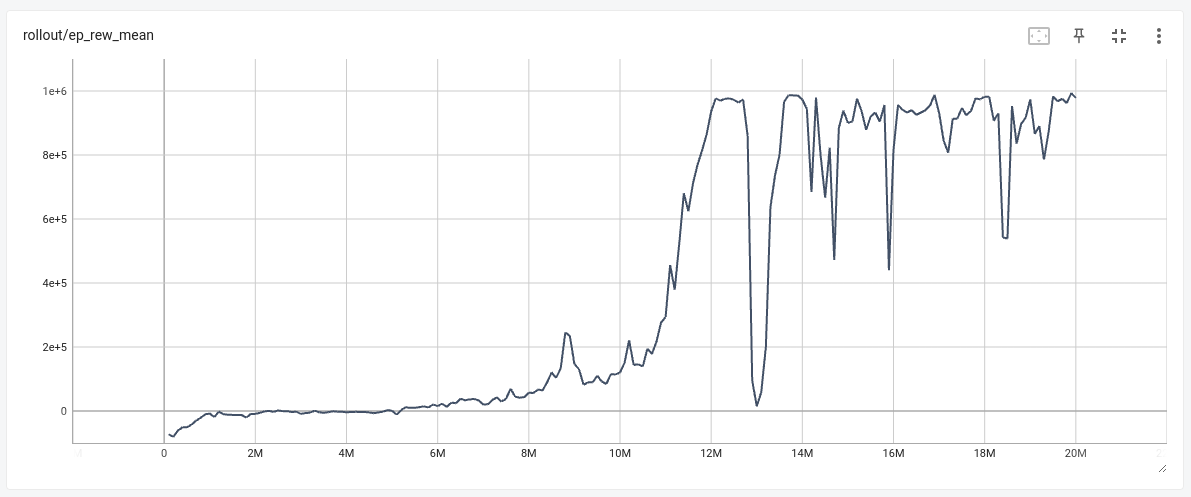
\includegraphics[width=0.9\textwidth]{figures/learning_curve/pendubot_learning_curve.png}} % First image
    \caption{pendubot learning curve}
    \label{fig:image_a}
\end{figure}

\begin{figure}[htbp]
    \centering
    \fbox{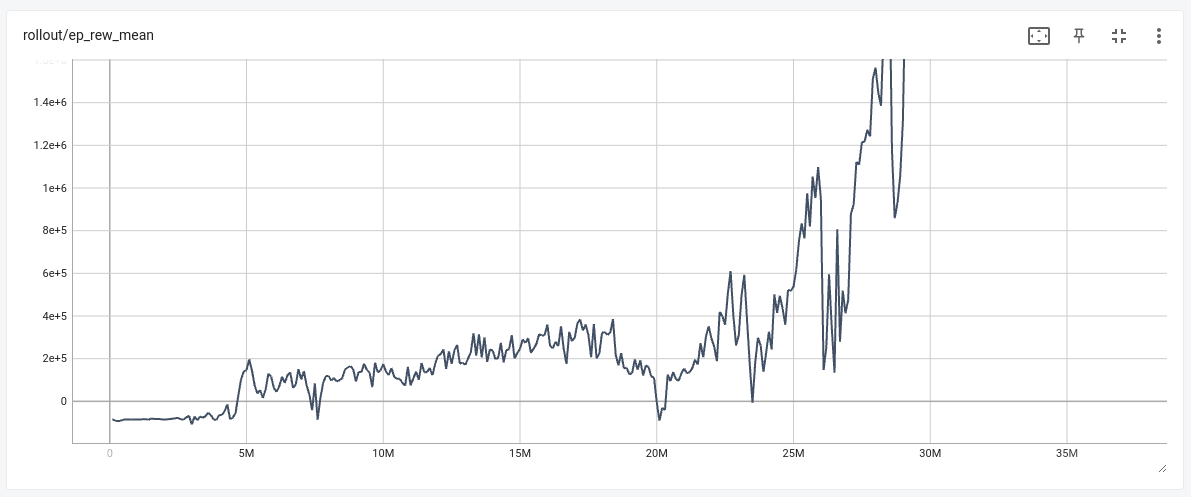
\includegraphics[width=0.9\textwidth]{figures/learning_curve/acrobot_learning_curve.png}} % Second image
    \caption{acrobot learning curve}
    \label{fig:image_b}
\end{figure}

\section{Simulation results}
This section is about simulation results in pendubot and acrobot.
\subsection{pendubot}
pendubot:
\begin{figure}[htbp]
    \centering
    \fbox{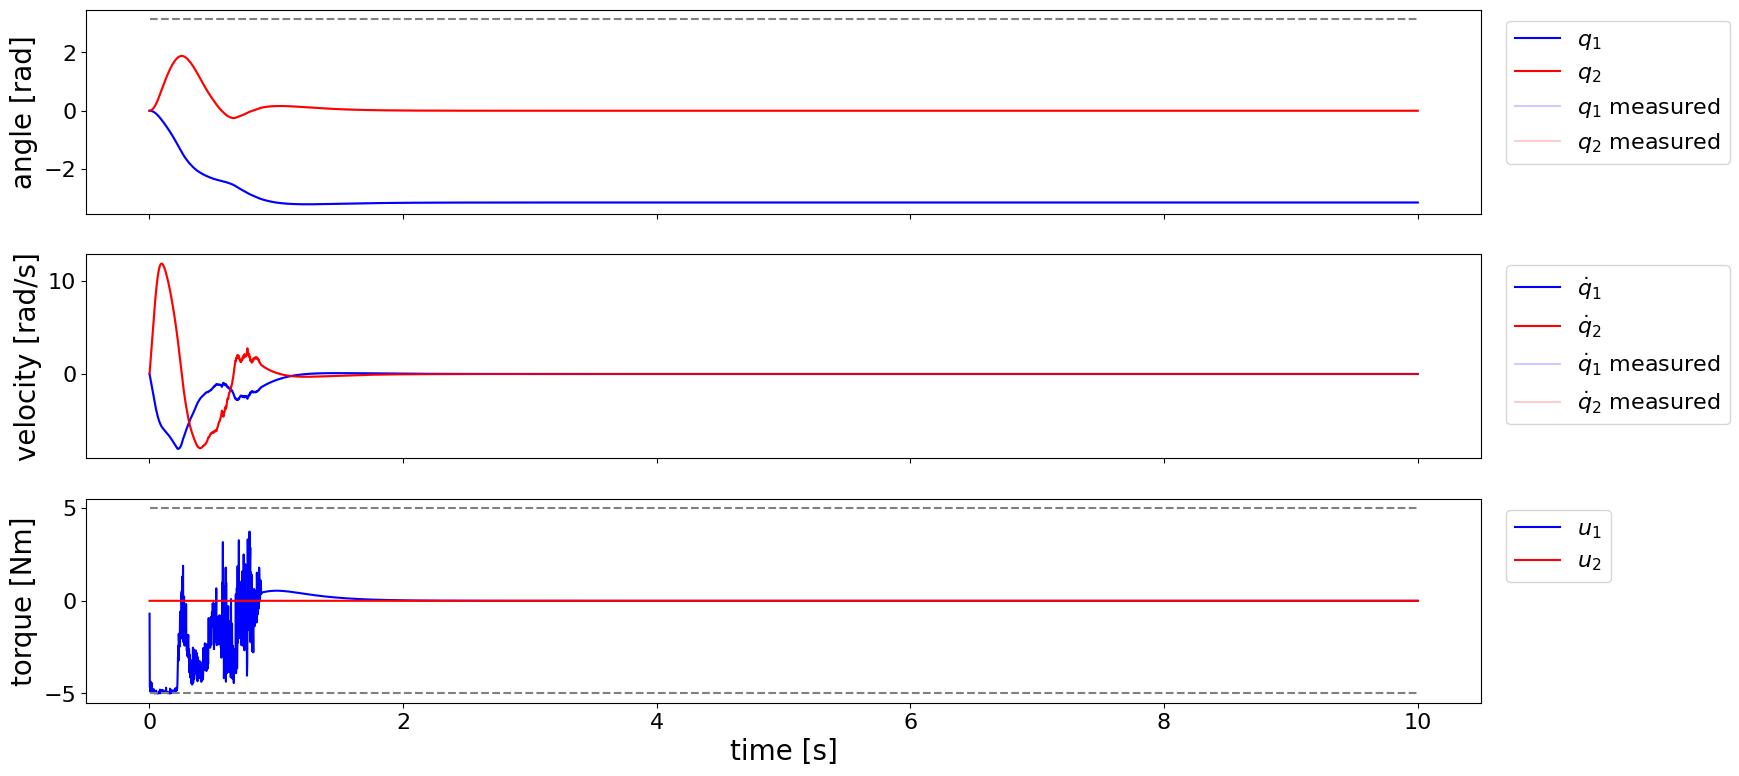
\includegraphics[width=0.9\textwidth]{figures/simulation_result/pendubot_unclipped.png}} % First image
    \caption{pendubot simulation result}
    \label{fig:image_a}
\end{figure}

\subsection{acrobot}
acrobot:
\begin{figure}[htbp]
    \centering
    \fbox{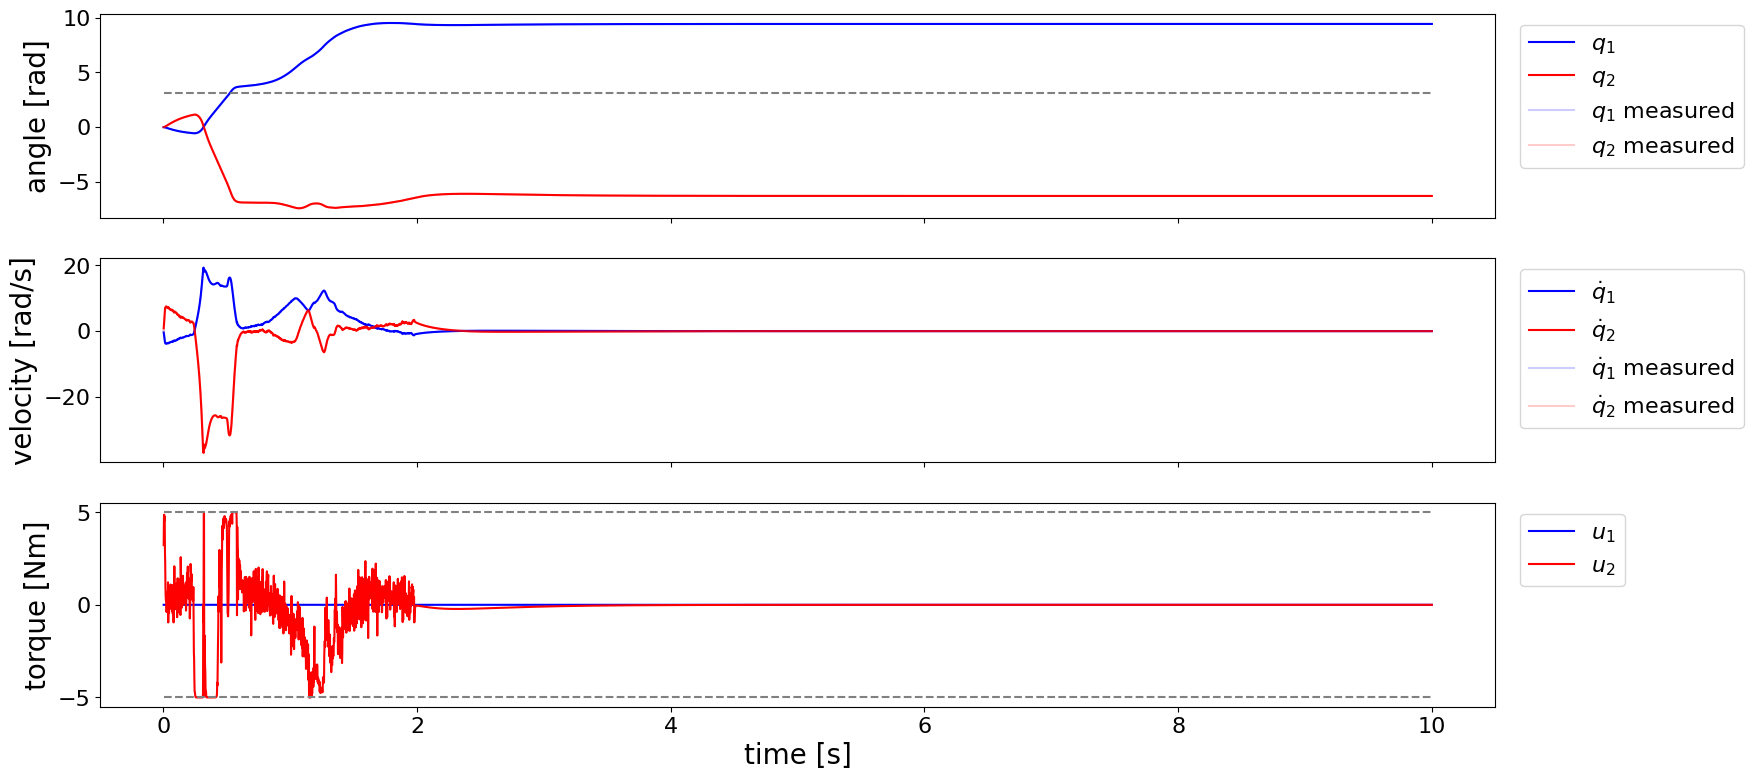
\includegraphics[width=0.9\textwidth]{figures/simulation_result/acrobot_unclipped.png}} % Second image
    \caption{acrobot simulation result}
    \label{fig:image_b}
\end{figure}


\cleardoublepage
